% Use only LaTeX2e, calling the article.cls class and 12-point type.

\documentclass[12pt]{article}

% Users of the {thebibliography} environment or BibTeX should use the
% scicite.sty package, downloadable from *Science* at
% www.sciencemag.org/about/authors/prep/TeX_help/ .
% This package should properly format in-text
% reference calls and reference-list numbers.

\usepackage{scicite}

% Use times if you have the font installed; otherwise, comment out the
% following line.

\usepackage{times}
\usepackage{graphicx}

% The preamble here sets up a lot of new/revised commands and
% environments.  It's annoying, but please do *not* try to strip these
% out into a separate .sty file (which could lead to the loss of some
% information when we convert the file to other formats).  Instead, keep
% them in the preamble of your main LaTeX source file.

% The following parameters seem to provide a reasonable page setup.

\topmargin 0.0cm
\oddsidemargin 0.2cm
\textwidth 16cm 
\textheight 21cm
\footskip 1.0cm

%The next command sets up an environment for the abstract to your paper.

\newenvironment{sciabstract}{%
\begin{quote} \bf}
{\end{quote}}

% If your reference list includes text notes as well as references,
% include the following line; otherwise, comment it out.

\renewcommand\refname{References and Notes}

% The following lines set up an environment for the last note in the
% reference list, which commonly includes acknowledgments of funding,
% help, etc.  It's intended for users of BibTeX or the {thebibliography}
% environment.  Users who are hand-coding their references at the end
% using a list environment such as {enumerate} can simply add another
% item at the end, and it will be numbered automatically.

\newcounter{lastnote}
\newenvironment{scilastnote}{%
\setcounter{lastnote}{\value{enumiv}}%
\addtocounter{lastnote}{+1}%
\begin{list}%
{\arabic{lastnote}.}
{\setlength{\leftmargin}{.22in}}
{\setlength{\labelsep}{.5em}}}
{\end{list}}

% Include your paper's title here

\title{Classification of X-Ray Images Using Various Features and Models}

% Place the author information here.  Please hand-code the contact
% information and notecalls; do *not* use \footnote commands.  Let the
% author contact information appear immediately below the author names
% as shown.  We would also prefer that you don't change the type-size
% settings shown here.

\author
{Mike Grimes\\
\\
\normalsize{Department of Computer Science, Michigan Technological University}\\
\normalsize{ImageCLEF 2015 - Medical Clustering Submission}\\
\\
\normalsize{magrimes@mtu.edu}
}

% Include the date command, but leave its argument blank.

\date{}

%%%%%%%%%%%%%%%%% END OF PREAMBLE %%%%%%%%%%%%%%%%

\begin{document} 

% Double-space the manuscript.

\baselineskip24pt

% Make the title.

\maketitle 

% Place your abstract within the special {sciabstract} environment.

\begin{sciabstract}
Using a training set of 500 X-Ray images preclassified with single class membership,
both linear and kernelized SVMs were trained using SIFT, SURF, and HoG features. Several
parameters were tuned and data collected on their effect on training, validation, and
testing error. Overall, on a set of 250 X-Ray images belonging to multiple classes,
a total classification rate of 70\% was attained.
\end{sciabstract}

Initially, the first checkpoint was to get a simple kernelized
SVM classifying the SIFT features of the unprocessed, unscaled
images. This first classification attempt used the {\it libsvm}
C-Support Vector Classifier implementation supplied as part of
the {\it sklearn} python module, and the {\it OpenCV} SIFT implementation.
With SIFT descriptors grouped into a histogram "bag-of-words" style,
by first k-means clustering ($k = 100$) a random sampling of 75\% of
the entire test data set, and then fitting the training data
SIFT descriptors into a histogram of the closest means.
Without tuning the $C$ and $\gamma$ parameters of the SVM and the
built-in RBF kernel, and using a k-fold cross-validation ($k = 5$)
and random shuffling of data, a training error rate of 0.25\% and
a validation error rate of 75.75\% were attained.

\section*{Tuning of $C$ and $\gamma$}

Obviously those error rates can be improved upon. Running the same
configuration with the different combinations of $C$ values from the range
$0.01$ to $1 * 10^{8}$ and $\gamma$ values from the range of $1 * 10^{-5}$
to $1000.0$ allowed for a visualization of classification performance.
\vspace{0.2in}

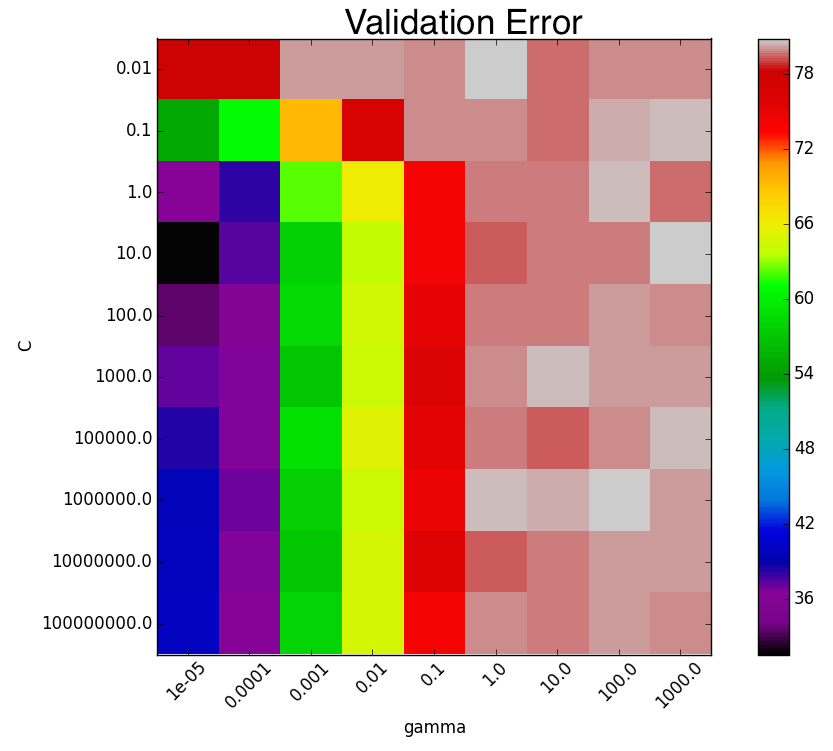
\includegraphics[scale=0.35]{../figures/val_c_gamma_chart.png}
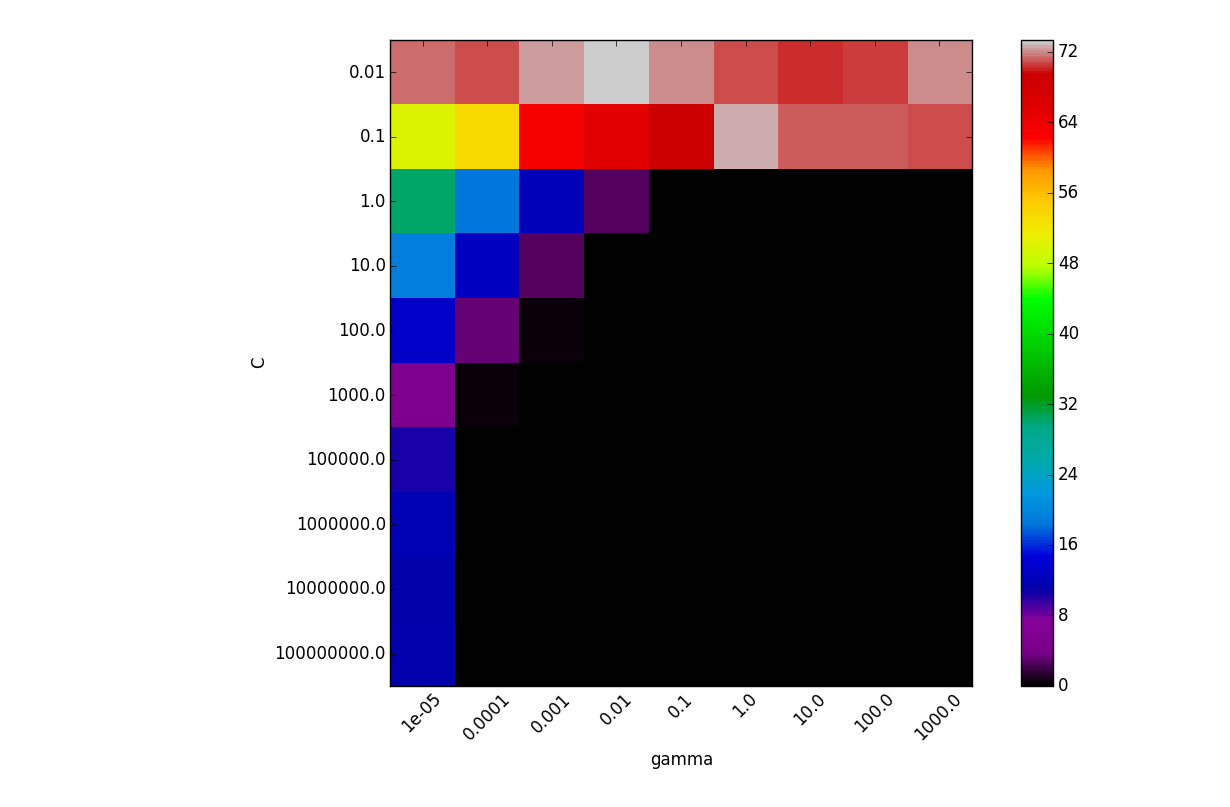
\includegraphics[scale=0.335]{../figures/train_c_gamma_chart.png}

By tuning the $C$ value for the SVM and the $\gamma$ parameter of the
RBF kernel as shown, a massive improvement on classification rate was
acheived: 0.4625\% and 36.25\% for training and validation error,
respectively.



\section*{Using a Different $k$ and SURF}

Upping the $k$ for the k-means clustering of the original 75\% of the
training data yielded no improvement on training or validation error:
1.388\% training error, and 37.92\% validation error. Although, swapping
out the SIFT descriptors for SURF descriptors did improve classification
rates quite a bit: 0.0\% and 30.396\% training and validation errors,
respectively

\section*{HoG and Image Scaling}

Histogram of Orientated Gradients is a widely used and extremely well-liked
feature detection method. While this does bring more parameters into play, they
can fairly easily be tuned to improve performance.

One downside to HoG is that when used with small cell and block sizes, the
gradient calculation can become quite CPU intensive, and the HoG can output
an extremely high-dimensional feature vector. With 1600x2500 images, 4x4 pixels
per cell, and 1x1 cells per block the feature vector consited of over 800,000
dimensions. Obviously, as soon as you get over more than a few data points with
dimensionality this high, fitting the SVM to the training data becomes very time
consuming as well.

Because of this large rise in data dimensionality, I decided to scrap the kernelized
SVM and stick with a linear-SVM for two reasons. First, calculating the kernel matrix
of this high dimensionality data would be absolutely horrendous. Just trying it and
letting it run for a few minutes quickly ate up the 8GB of memory in my laptop. Second,
with data that has this many dimensions, introducing more through the use of a kernel
doesn't seem like it would be very effective.

Similar to how the $C$ and $\gamma$ parameters were tuned earlier, I ran a combination
of a number of pixel-per-cell and cells-per-block parameters to find one that
improved my classification rate the most.

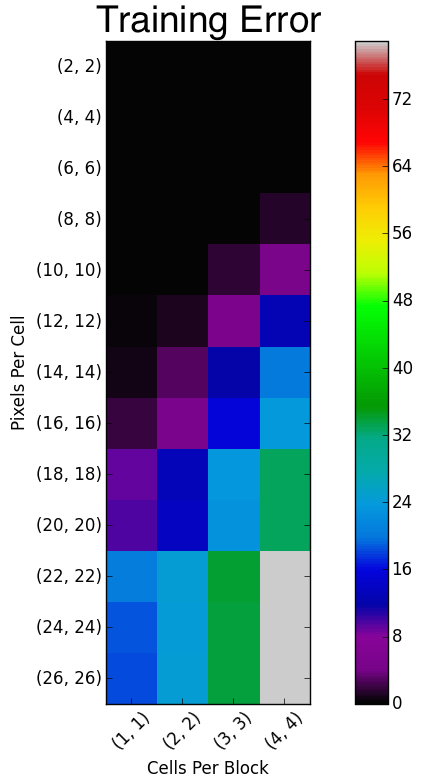
\includegraphics[scale=0.5]{../figures/train_hog_params.png}
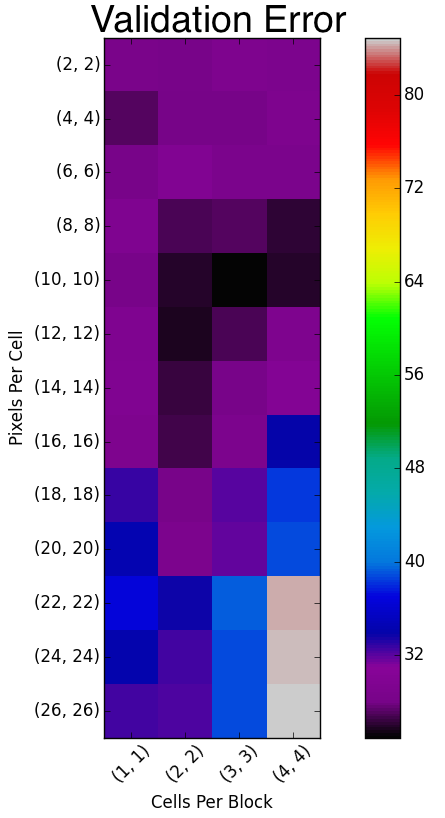
\includegraphics[scale=0.48]{../figures/val_hog_params.png}

As can be seen, there's a nice dip in the validation error rate when the pixels-per-cell
is 10x10 and the cells-per-block are 3x3. This brought yet another large gain in
classification performance: 1.62\% training error and 24.9\% validation error.

\section*{Testing Data and Multi-Membership Predictions}

Testing data consisted of 250 unclassified images of widely varying sizes,
and of what seemed to be much lower quality than the training data. Many
images have large white areas surrounding the edges, are of varying levels
of darkness, and contain many images of bones with metal fixtures like screws
and bolts in them. Alongside the X-rays of people there are "True Negatives", or
X-rays of electronics, tools, or nothing at all. Sometimes these contain letters
in them, such as a single "R", as seen below. I really expected this to throw off
the classifier, and result in a throughly crappy testing rate. To my surprise, this
was not the case.

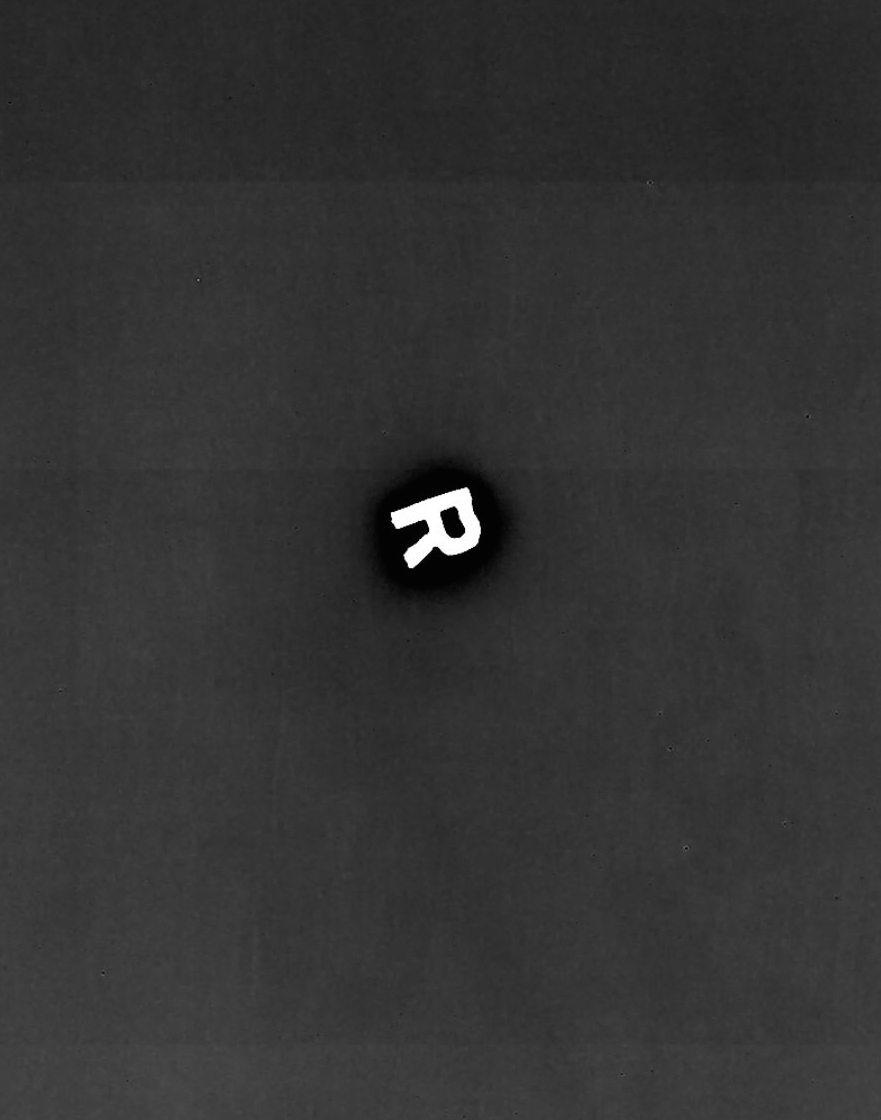
\includegraphics[scale=0.14]{../figures/letter-r.png}
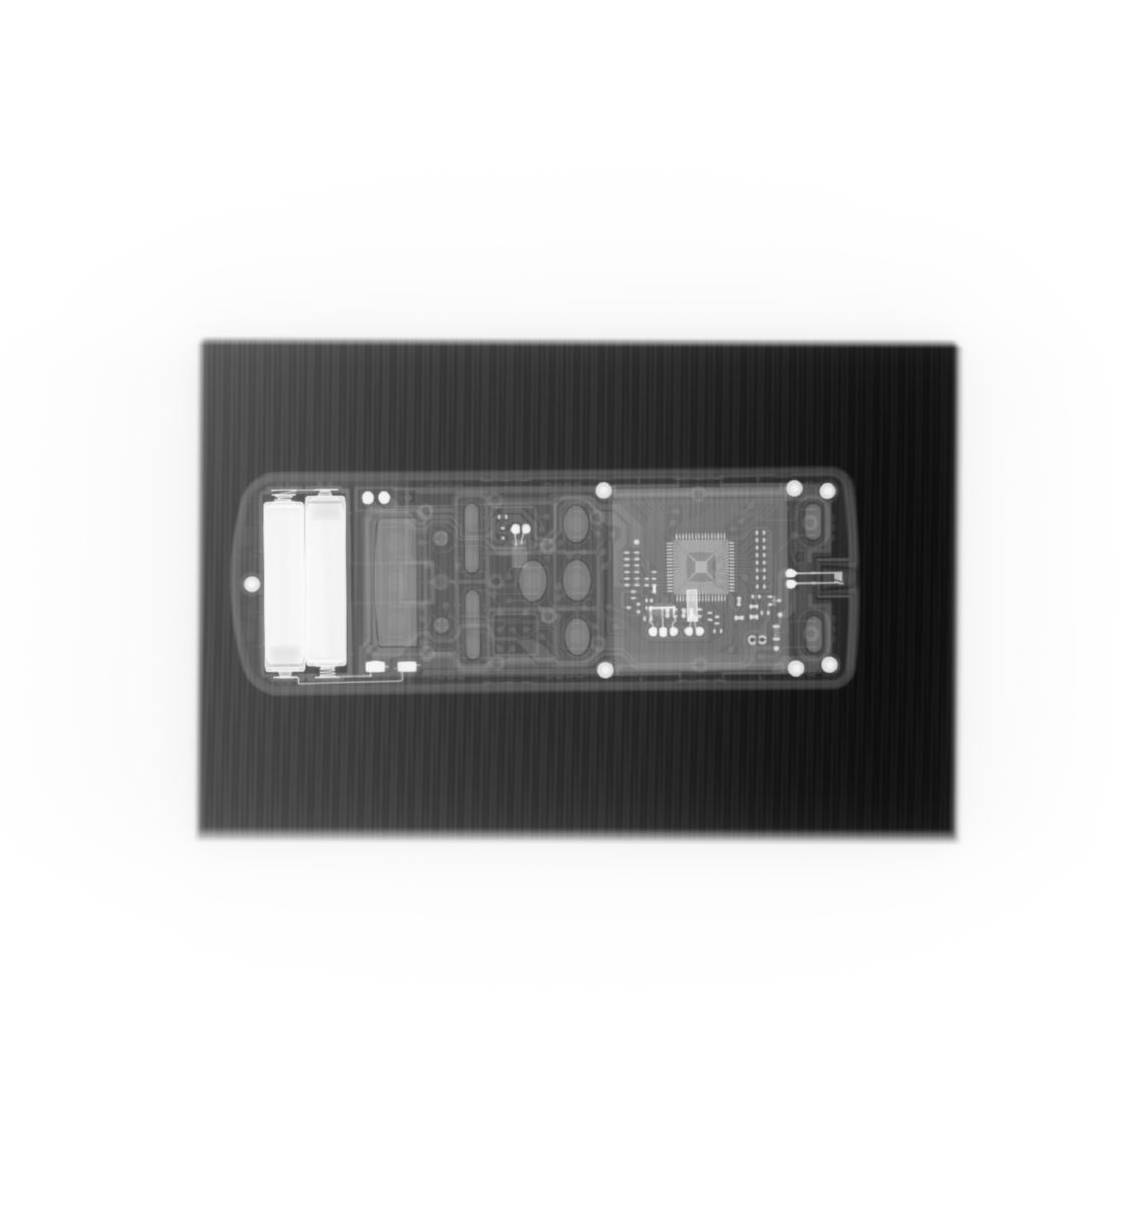
\includegraphics[scale=0.14]{../figures/phone.png}
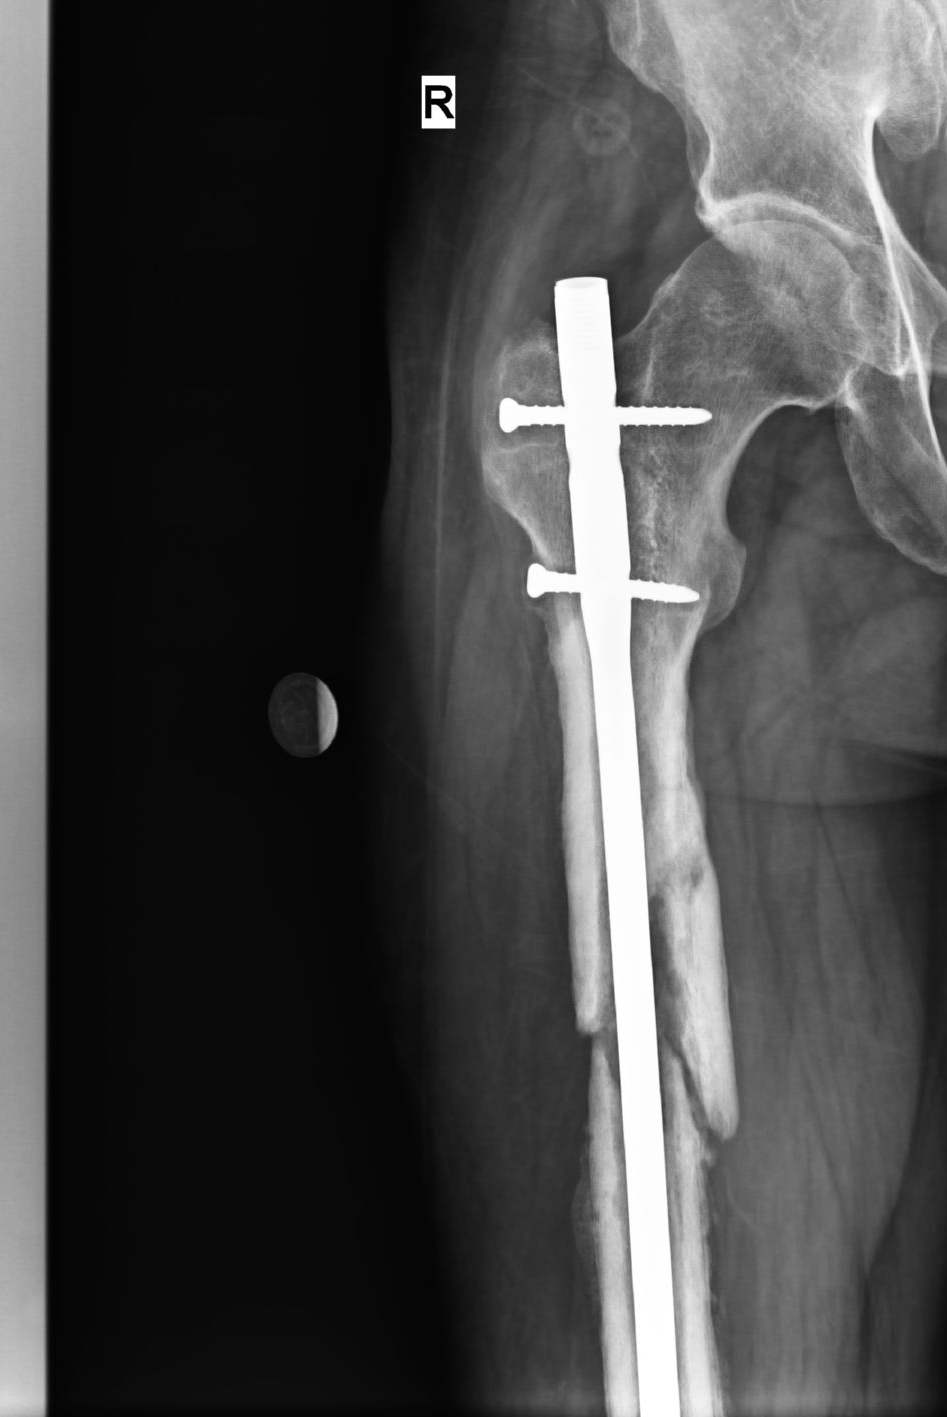
\includegraphics[scale=0.14]{../figures/leg-bolt.png}

\vspace{0.2in}

I hand-classified the 250 images, with some images belonging in up to 3 classes.

Here, I also switched the SVM to the liblinear implementation, instead of the
libsvm one, as it provides a probability prediction, instead of just a straight
one-class prediction.

In order to deal with the prediction multiple classes, I decided that a threshold
of 25\% probabilty seemed to be a reasonable cutoff for class-decidingship. When
a prediction is made on a dataset, the SVM outputs a vector of $K$ probabilities,
where $K$ is the number of classes being classified for. As you probably guessed,
these probabilities all add up to $1$. My thinking was that even if the SVM classified
images perfectly, there would never be any way for an image to be in more than 4
classes (full-body X-ray). Unless, perhaps, someone took one while holding a wrench,
or an old VCR.

Next, there was the problem of calculating the number of correct classifications. My
intuition was to check each output class from the SVM that made the probability
threshold, and if that class was in the testing label for that image, I added
$\frac{1}{n}$ to the number of correct guesses, where $n$ is the number of classes in
the testing label for the image. So for example, if a class label of $1$ is output
for an image, and the only class in the label for that image is $1$, then the
number of correct guesses is incremented by $1$. Or, if a class label of $2$ is
output for an image, and the class labels for that image are $0$, $2$, and $4$,
the number of correct guesses is incremented by $\frac{1}{3}$. Notice, this
does not penalize incorrect classifications, so technically classifying each image
as all classes would result in 100\% classification accuracy. Obviously this isn't
what the SVM does, but it should be taken into mind.

So here are the rates of the {\it liblinear} SVM: 6.03\%, 27.06\%, and 28.616\%
for training, validation, and testing errors, respectively.

\section*{Testing Error for Previous Methods}
For some reason, the SURF and SIFT with $k = 200$ k-means, and multiclass
prediction absolutely murders the testing classification rate. 0.0\% training error,
27.19\% validation error and 70.813\% testing error for SURF. SIFT is a bit worse:
1.083\%, 35.438\%, and 71.636\% for training, validation, and testing error rates,
respectively. I'm not entirely sure what the reason is for this, since the validation
doesn't do a whole lot worse than it does for the HoG.

\section*{Additional Thoughts}
So there were quite a few things I wanted to try, but never got around to. One idea
as to why SURF and SIFT perform so poorly on the test set is that the way that they
pull features from the image may be more affected by artifacts of the images, such
as white spots, metal objects, and labels on the image. If I had more time I would
have filtered keypoints from the SURF and SIFT descriptors that fall on those rectangle
labels. More pre-processing and normalizing of the images would probably give some
pretty large benefits, too.

\section*{Conclusion}
All in all, mediocre classification can be done with a simple SVM and feature detection
such as SIFT or SURF. HoG took a bit more work in order to get the feature vectors
all the same size, but its still a very easy feature detection method to get working.
It's also easy to see that fine tuning of model and feature detection parameters can
have some large payoffs.

\section*{References}

\vspace{0.2in}

Sci-kit Pyton Image Processing Library {\em http://scikit-image.org/docs/dev/api/skimage.html}

\vspace{0.2in}

OpenCV {\em http://opencv.org}

\vspace{0.2in}

My Github, with code {\em http://github.com/magrimes/medical-clustering}

\end{document}
